\chapter{Asking Scottsdale Millionaires How They Got Rich}

We begin with a lecture that arrives in the form of street interviews but organizes itself around a surprisingly stable mathematical spine. Wealth is not treated merely as possession. It is described through cash timing, margin, leverage, compounding, purchasing power, and the difference between a friendly seller and a trusted one. These notes follow the order of the School of Hard Knocks interview and preserve its movement from teaser claim to concrete mechanism, with the series curation carried by LazyingArt LLC.

\section{Cold Open and the Scottsdale Premise}

The lecture opens by announcing conclusions before it has earned them. This is not yet derivation; it is foreshadowing. We are shown eight-figure businesses, large revenue targets, and a compounding metaphor, all before the fieldwork has properly begun. The effect is to tell us, at once, what kinds of quantities will matter.

\begin{equation}
(R_{\text{last}},R_{\text{goal}},R_{+4y}) = (160\,\text{M}, 250\,\text{M}, 1\,\text{B})
\end{equation}

\begin{equation}
a_n = 0.01 \cdot 2^{n-1}
\end{equation}

The first equation is not a proof, only a growth ladder stated in the teaser. The second is the lecture's compounding image: a penny doubled daily. We should hear both as promises of later mechanism. Only after that does the speaker reset the scene and tell us what the experiment is. Scottsdale is introduced as one of the wealthiest cities in the United States, and the inquiry is framed simply: go to the operators, ask what they do, and make the path to wealth legible.

That reset matters. The chapter should not read like a bag of quotes. It should read as an inquiry into how these claims are supposed to hold together.

\section{Revenue, Profit, and the Cash-Poor Paradox}

The first major interview does something essential. It breaks the glamour of large numbers before the chapter has time to become naive about them. We are told of an entrepreneur making tens of millions and yet becoming nearly insolvent at the level that matters most urgently: tomorrow morning.

\begin{definition}
Let \(C_{\text{due}}\) denote immediate obligations due by the next day, \(B\) the cash balance on hand, and
\[
L_{\text{gap}} = C_{\text{due}} - B
\]
the short-term liquidity gap.
\end{definition}

\subsection{Question \& Answer}

\paragraph{Question.} How can someone who is doing large business still find himself in a state of panic over next-day cash?

\paragraph{Answer.} Because revenue, profit, and cash timing are not the same object.

The lecture gives us enough numbers to make the pressure visible.

\begin{align}
C_{\text{due}} &\approx 550{,}000 + 200{,}000 = 750{,}000,\\
B &\approx 300{,}000,\\
L_{\text{gap}} &\approx 750{,}000 - 300{,}000 = 450{,}000.
\end{align}

This is the worked arithmetic example that turns a dramatic story into a concrete mechanism. The entrepreneur has an account balance, yes, but the balance is measured against a much larger next-day obligation stream. The lecture's memorable slogan, ``revenue is for vanity, profit is for sanity,'' already points in the right direction, but the crisis itself reveals a third term: liquidity arrives on a schedule.

The resolution is equally concrete. The speaker returns to a mentor's line, ``sales cures everything,'' and what follows is not mysticism but a sequence: rally the team, create a new offer, launch quickly, ask for time, and sell out of the hole.

\begin{equation}
S_{\text{new}} \approx 800{,}000 > L_{\text{gap}}.
\end{equation}

The point is not that sales literally cures every problem. The point is that it can rapidly transform persuasion into cash commitments, and that cash, arriving in time, can outrun fixed obligations that otherwise break the firm. The lecture begins here because it wants to puncture the childish idea that a large revenue headline means automatic financial ease.

\section{From Rescue to Leverage: Sales, Real Estate, and Team Design}

Once the lecture has shown us sales as a rescue mechanism, it widens the frame. Sales is no longer merely the emergency pump that keeps the organism alive. It becomes the portable skill that can be carried into a more durable architecture of wealth.

\begin{definition}
In the lecture's usage, the single-tenant triple-net lease game means owning the property while a high-credit tenant occupies it and carries most operating obligations.
\end{definition}

The speaker recommends this not as a romantic theory of land, but as a business structure: own the building, place a strong tenant inside it, and let the tenant quality stabilize the income stream. The examples are concrete and deliberately ordinary: CVS, Walgreens, a doctor's office. The building matters less as architecture than as a container for predictable payment.

Several claims are then placed side by side:
\begin{itemize}
\item Sales is the skill that first opens the door.
\item Real estate is the asset that can hold value and payments over time.
\item Larger commercial deals may be easier than smaller ones because institutions process them through checklists rather than improvisation.
\item A founder does not reach eight figures by remaining the irreplaceable bottleneck.
\end{itemize}

The lecture's line ``I fired myself'' is not self-erasure. It is an organizational statement. The founder's task is to build a team that is better than his own improvisational reflexes. ``Money loves speed'' follows naturally. A system with good people and a clear checklist moves faster than a founder-centered operation that depends on personality.

\section{Blue-Collar Scale, Margin, and Bought-Back Time}

The next interview shifts register. We move from the emotional crisis of an entrepreneur's cash shortage to the colder arithmetic of a large home-service business. This is important to the lecture's logic. We are no longer asked to admire intensity. We are asked to see scale as something operational.

If revenue is \(R\) and profit margin is \(m\), then the standard identity is

\begin{equation}
\Pi = R\,m.
\end{equation}

The speaker says the company will do about \(240\,\text{M}\) this year and is over \(20\%\) on the bottom line. If we treat that only as an approximate margin statement, we obtain

\begin{equation}
R \approx 240\,\text{M}, \qquad m > 0.20
\quad \Longrightarrow \quad
\Pi > 48\,\text{M}.
\end{equation}

\begin{remark}
The phrase ``over \(20\%\) of the bottom line'' is colloquial and not strict accounting language. We use the inequality only as a rough reconstruction of the lecture's margin logic.
\end{remark}

The next mechanism is purchasing power. The business buys so many doors and parts that it pays less than a smaller operator would pay. In compact form the claim is this:

\begin{equation}
q_2 > q_1 \quad \Longrightarrow \quad c_{\text{unit}}(q_2) < c_{\text{unit}}(q_1).
\end{equation}

This is not a detailed cost curve; the lecture does not give us one. But it does give the direction clearly enough. Scale is not merely more work. Scale changes the price at which the business itself buys.

From here the interview pivots into time leverage. ``Buy back your time'' is the phrase. Some people, the speaker says, can buy back thirty hours a week and then compound their time.

\begin{equation}
T'_{\text{available}} = T_{\text{available}} + T_{\text{freed}},
\qquad
T_{\text{freed}} \approx 30\ \text{hr/week}.
\end{equation}

Again the lecture is metaphorical in part. No one has created more than a week. But the founder reallocates hours away from low-value activity and toward strategic work. That change in allocation behaves like leverage.

The lecture then makes an interesting sociological split. Millionaires are described through habits: early rising, cold plunges, family discipline. Billionaires are described through networks and judgment: knowing who to call, paying for the best, refusing to haggle over quality. What follows is a still narrower triad, almost a moral version of control theory:
\begin{enumerate}
\item focus on what one has, not only what one lacks;
\item focus on today and the future, not the past;
\item focus on what one can control, not what lies outside one's control.
\end{enumerate}

This is not mathematics in a formal sense, but it is sequenced as a control problem. Attention is treated as a scarce resource, and misallocated attention is treated as a real source of stagnation.

\section{Family Capital Formation as a Small-Scale Compounding Mechanism}

The sponsor segment arrives during travel, but it should not be discarded as dead matter. Structurally it translates the lecture's compounding logic from business scale to household scale. The same idea reappears in a different register: small present inputs, if routed through the right account, can become future optionality.

\begin{figure}[h]
\centering

\includegraphics[width=0.92\textwidth]{lecture_76_figure_02.png}
\caption{Fabric by Gerber Life gift-card mockup used to illustrate birthday contributions into a child investment flow.}
\end{figure}

The frame is worth keeping because it provides a concrete visible example. The app mockup shows a gift card addressed to Charlie, from Grandma and grandpa, with a visible contribution amount:

\begin{equation}
G = \$25.
\end{equation}

The lecture's more general investment logic can be written in standard future-value form. If \(c\) is the recurring contribution and \(r\) the period return, then

\begin{equation}
FV = \sum_{k=0}^{n-1} c(1+r)^k.
\end{equation}

We should be careful here. The screenshot itself gives us the visible one-time example \(G=\$25\). The transcript separately mentions the possibility of contributing as little as \(\$1\) a day, but that daily figure is transcript-backed rather than figure-backed. The mathematical point is still clear enough: the lecture wants gifts to stop behaving like consumption and start behaving like seeded capital.

A small schematic helps isolate the mechanism without replacing the original visual evidence.

\begin{figure}[h]
\centering
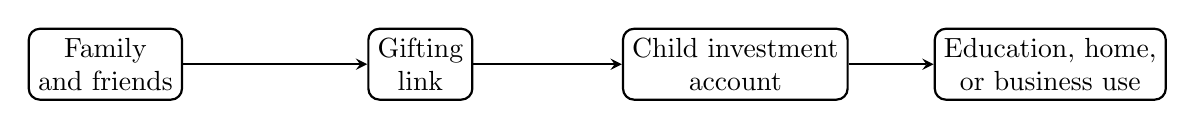
\begin{tikzpicture}[>=stealth, thick]
\node[draw, rounded corners, align=center] (a) at (0,0) {Family\\and friends};
\node[draw, rounded corners, align=center] (b) at (4,0) {Gifting\\link};
\node[draw, rounded corners, align=center] (c) at (8,0) {Child investment\\account};
\node[draw, rounded corners, align=center] (d) at (12,0) {Education, home,\\or business use};
\draw[->] (a) -- (b);
\draw[->] (b) -- (c);
\draw[->] (c) -- (d);
\end{tikzpicture}
\caption{A cleaned schematic of the mechanism implied by the sponsor segment.}
\end{figure}

The lecture is making a quiet but serious claim here: family finance can be understood as capital formation if the channel is right.

\section{Trust, Liking, and the Logic of Purchase}

The later G-Wagon interview corrects a sales slogan that is repeated so often it has hardened into folklore. The lecturer cites an older maxim, ``people buy from people they like,'' only to narrow it sharply.

\subsection{Question \& Answer}

\paragraph{Question.} Do people really buy from people they like?

\paragraph{Answer.} Not primarily. They buy from the person or company they trust to produce the best result.

Let \(E_i\) denote the buyer's expected result from seller \(i\). Then the lecture's logic can be written as

\begin{equation}
\text{Choose } A \text{ over } B \text{ if } E_A > E_B;
\qquad
\text{use liking only when } E_A = E_B.
\end{equation}

This is a helpful formalization because the lecture insists on a boundary condition: ``if all things are equal.'' That clause matters. It demotes personal affection from governing principle to tie-breaker. We are not asked to become hostile. We are asked to become precise.

The examples are memorable because they are domestic rather than abstract. One may love grandma and still buy from a stranger if one trusts the stranger to do the job better. One may have a friend with a local hardware shop and still purchase from Amazon if Amazon is trusted to deliver the better result. The correction is therefore not sentimental. It is a decision rule.

What the lecture is after is commercial seriousness. Trust is operational. Liking is supplementary.

\section{Sales as the Lowest-Barrier Wealth Engine}

The final movement of the lecture takes the earlier claims about sales and pushes them toward a general theory of ascent. Sales is described not only as useful, but as the lowest-barrier path into large earnings. That claim is sharpened by comparison with a professional route like medicine: many years of school, large debt, residency, modest earnings for a long interval, and only then the possibility of substantial income.

Against that, the lecture places a rapid income ladder:

\begin{equation}
(I_1, I_2, I_3) = (125\text{k}, 225\text{k}, 500\text{k}).
\end{equation}

This sequence is not presented as a universal law. It is autobiographical evidence offered in support of a broader proposition: one can enter sales with very little formal barrier and move quickly if the skill is mastered.

The compounding metaphor returns here, this time not as an isolated teaser but as part of a more general rhetoric of acceleration. A social media example is used to show that growth can feel slow until it stops being slow. One million followers may take a year; the next million may take ninety days. The mathematical object is still the same one we saw earlier: nonlinear growth.

The lecture also turns pain into a kind of commercial mechanics. The tennis-ball image, called ``bounce-ology,'' should not be over-formalized, but its meaning is plain enough. Hardship stores pressure. Once the person acts, that stored pressure can become upward motion. So too the slogan ``when the pain overrides the fear of change, people change.'' We are being given, not a theorem, but a law of motivational dynamics.

The same section then provides a practical triad for getting wealth in today's world:
\begin{enumerate}
\item be fully committed;
\item develop the right skills;
\item build a culture in which the surrounding people share the same mission.
\end{enumerate}

From there the lecture narrows one last time to the ethics of sales itself. The central line is that the seller must care more about the client than the client cares about himself. This is joined to another rule: be where your feet are. Attention is treated not as etiquette but as force. Presence is part of what persuades.

The close is deliberately wider than business technique. We are asked whether the whole undertaking is worth it, and the answer is yes, because the true loss is not merely low income. The true loss is the unlived life, the life one was capable of inhabiting but did not have the courage to attempt. That is the lecture's last escalation. It ends not with a spreadsheet but with a demand for agency.

\section{Summary}

The lecture's surface is informal, but its internal structure is disciplined. It begins with headline numbers, then forces us to distinguish revenue from profit and both from cash timing. It widens from survival to leverage through sales, real estate, margin, scale purchasing, and delegation. It briefly translates compounding into family finance, then sharpens sales theory by replacing liking with trust in results. Finally, it argues that sales remains the lowest-barrier engine of ascent, provided it is joined to commitment, skill, culture, and real care for the client.

The resulting chapter is not about luxury goods. It is about mechanisms: how money arrives, how it scales, how it gets trapped, and how it can be made to move again.